\chapter{ANALISIS DAN PERANCANGAN SISTEM}
\section{Analisis Sistem}
\tab Pada bab ini akan dijelaskan mengenai tahapan dalam membangun sistem berbasis \textit{Internet of Things} "EasyMeeting", yakni menganalisis sistem yang akan dibangun. Analisis sistem dijelaskan dalam tiga sub-bagian, yakni deskripsi umum sistem, fungsi produk, dan analisis kebutuhan.

\subsection{Deskripsi Umum Sistem}
\tab Secara umum, sistem "EasyMeeting" adalah sebuah sistem berbasis \textit{Internet of Things} yang berfungsi untuk membantu persiapan ruang rapat di PT Telekomunikasi Indonesia (Telkom) supaya lebih efisien.\\
\tab Sistem "EasyMeeting" terdiri dari 3 komponen, yakni aplikasi \textit{client}, \textit{server}, dan \textit{microcontroller}. Aplikasi \textit{client} didesain berbasis \textit{mobile} dengan memanfaatkan bot API dari aplikasi \textit{messaging} yang sedang tenar, yakni Telegram dan Telegram Bot API. \\
\tab Komponen \textit{microcontroller} yang digunakan untuk membangun sistem ini adalah Arduino UNO, DHT11, \textit{breadboard}, resistor, \textit{jumper wires}, LED \textit{light bulb}, \textit{infrared sensor module} dan \textit{infrared receiver module}. Komponen-komponen tersebut dirangkai dan diprogram sedemikian rupa hingga sesuai dengan kebutuhan. Program \textit{microcontroller} diletakkan pada sebuah \textit{host} yang berperan sebagai \textit{server}, kemudian program di-\textit{compile} dan dijalankan menggunakan Arduino IDE.

\subsection{Fungsi Produk}
\tab Sistem "EasyMeeting" memiliki beberapa fungsi utama sebagai berikut:
\begin{enumerate}
	\item Dapat menyalakan lampu dan AC ruangan
	\item Dapat mematikan lampu dan AC ruangan
	\item Dapat menampilkan status kondisi lampu dan AC ruangan
	\item Dapat menampilkan suhu ruangan
\end{enumerate}

\subsection{Analisis Kebutuhan}
\tab Sistem "EasyMeeting" yang dibuat harus mampu memenuhi beberapa fungsi utama yang telah dijelaskan. Fungsi-fungsi ini merupakan hasil analisis kebutuhan yang telah dilakukan di PT Telekomunikasi Indonesia (Telkom), khususnya pada Divisi \textit{Information Technology}. Analisis kebutuhan dibagi menjadi dua, yakni kebutuhan fungsional dan kebutuhan non-fungsional.

\subsubsection{Kebutuhan Fungsional}
\tab Kebutuhan fungsional menjelaskan bagaimana sistem "EasyMeeting" bekerja. Tabel \ref{table:kebutuhan_fungsional} menjelaskan kebutuhan fungsional dari sistem "EasyMeeting".

\begin{table}[H]
	\centering
	\begin{tabular}{ | p{3cm} | p{6cm} | }
		\hline
		\textbf{Kode Kebutuhan} & \textbf{Deskripsi Kebutuhan} \\ \hline
		F-001 & Menyalakan lampu dan AC ruangan \\ \hline
		F-002 & Mematikan lampu dan AC ruangan \\ \hline
		F-003 & Melihat status kondisi lampu dan AC ruangan \\ \hline
		F-004 & Melihat suhu ruangan \\ \hline
	\end{tabular} \caption{Kebutuhan Fungsional}
	\label{table:kebutuhan_fungsional}
\end{table}

Penjelasan rinci dari masing-masing kebutuhan fungsional pada tabel \ref{table:kebutuhan_fungsional} dijelaskan sebagai berikut:
\begin{enumerate}
	\item \textbf{Menyalakan lampu dan AC ruangan} \\
	\tab Pengguna yang telah terotentikasi dan terotorisasi dapat menyalakan lampu dan AC dalam ruangan yang akan digunakan untuk rapat.
	\item \textbf{Mematikan lampu dan AC ruangan} \\
	\tab Pengguna yang telah terotentikasi dan terotorisasi dapat mematikan lampu dan AC dalam ruangan yang akan digunakan untuk rapat.
	\item \textbf{Melihat status kondisi lampu dan AC ruangan} \\
	\tab Pengguna yang telah terotentikasi dan terotorisasi dapat menampilkan kondisi lampu dan AC dalam ruangan rapat untuk mengecek apakah ruangan tersebut sedang digunakan atau tidak.
	\item \textbf{Melihat suhu ruangan} \\
	\tab Pengguna yang telah terotentikasi dan terotorisasi dapat melihat suhu dalam ruangan yang sedang digunakan untuk rapat.
\end{enumerate}

\subsubsection{Kebutuhan Non-Fungsional}
\tab Kebutuhan non-fungsional menjelaskan kebutuhan pengguna untuk mendefinisikan bagaimana batasan dan karakteristik dari sistem "EasyMeeting". Tabel \ref{table:kebutuhan_non_fungsional} menjelaskan kebutuhan non-fungsional dari sistem "EasyMeeting".

\begin{table}[H]
	\centering
	\begin{tabular}{ | p{3cm} | p{6cm} | }
		\hline
		\textbf{Kode Kebutuhan} & \textbf{Deskripsi Kebutuhan} \\ \hline
		NF-001 & Sistem beroperasi selama jam kerja \\ \hline
		NF-002 & Sistem dapat diakses dari mana saja selama jam kerja \\ \hline
		NF-003 & Sistem berjalan pada semua versi Telegram \\ \hline
		NF-004 & Pengguna yang dapat menggunakan sistem adalah pengguna yang sudah terotorisasi dan terotentikasi \\ \hline
		NF-005 & Pengguna harus menambahkan bot Telegram "EasyMeeting" sebelum dapat menggunakan sistem \\ \hline
	\end{tabular} \caption{Kebutuhan Non-Fungsional}
	\label{table:kebutuhan_non_fungsional}
\end{table}

\section{Perancangan Sistem}
\tab Pada bab ini akan dijelaskan mengenai perancangan sistem berbasis \textit{Internet of Things} "EasyMeeting", meliputi desain sistem secara umum dan desain sistem masing-masing fitur.\\
\tab Desain sistem dilakukan untuk mengetahui jalannya proses bisnis pada suatu aplikasi sehingga pengembang aplikasi dapat dengan mudah melakukan perubahan atau penyempurnaan. Desain sistem yang digunakan adalah \textit{use case diagram}, \textit{physical data model}, dan diagram aktivitas.\\
\tab \textit{Use case diagram} menunjukkan proses bisnis dan siapa saja yang terlibat pada proses tersebut seperti yang ditunjukkan pada Gambar \ref{figure:usecase}. \textit{Physical data model} akan memetakan bagaimana \textit{database} dibangun agar dapat digunakan dan diimplementasikan pada aplikasi. Terakhir, diagram aktivitas menunjukkan bagaimana sistem berjalan dan melakukan respon pada \textit{input} dari pengguna. Diagram aktivitas digunakan untuk menjelaskan setiap fitur di dalam sistem secara lebih detail.

\begin{figure}[H]
	\centerline {
		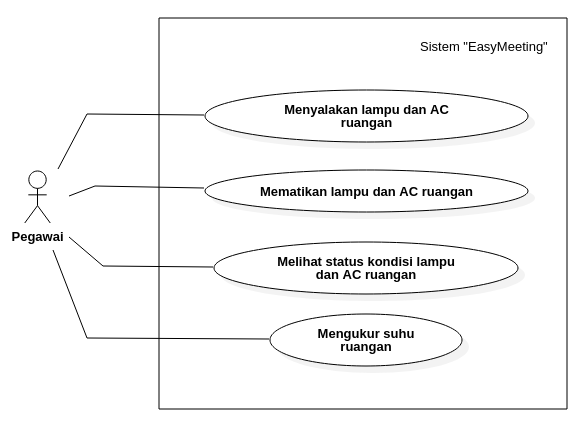
\includegraphics[width=\linewidth]{bab4/img/uc_diagram.png}
	}
	\caption{\textit{Use Case Diagram}}
	\label{figure:usecase}
\end{figure}

\subsubsection{Desain Sistem Menyalakan Lampu dan AC Ruangan}
\tab Pengguna yang dapat menggunakan fitur ini hanyalah pegawai Telkom dan admin sistem. Pengguna harus terlebih dahulu melakukan otentikasi dan otorisasi sebelum dapat menggunakan fitur untuk menyalakan lampu dan AC ruangan menggunakan perintah tertentu yang dapat dilihat dalam manual penggunaan bot. Diagram aktivitas pada gambar \ref{figure:activity_1} akan menjelaskan alur untuk menyalakan lampu dan AC ruangan secara lebih jelas.

\begin{figure}[H]
	\centerline {
		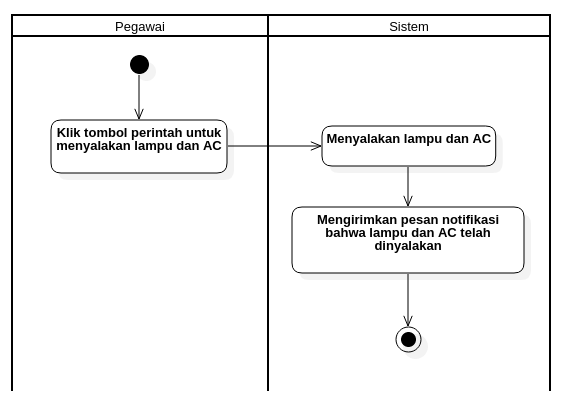
\includegraphics[width=\linewidth]{bab4/img/activity_diagram_menyalakan.png}
	}
	\caption{Diagram Aktivitas: Menyalakan Lampu dan AC Ruangan}
	\label{figure:activity_1}
\end{figure}

\subsubsection{Desain Sistem Mematikan Lampu dan AC Ruangan}
\tab Fitur ini juga hanya dapat diakses oleh pegawai Telkom dan admin sistem. Pengguna harus terlebih dahulu melakukan otentikasi dan otorisasi sebelum dapat menggunakan fitur untuk mematikan lampu dan AC ruangan menggunakan perintah tertentu yang dapat dilihat dalam manual penggunaan bot. Diagram aktivitas pada gambar \ref{figure:activity_2} akan menjelaskan alur untuk mematikan lampu dan AC ruangan secara lebih jelas.

\begin{figure}[H]
	\centerline {
		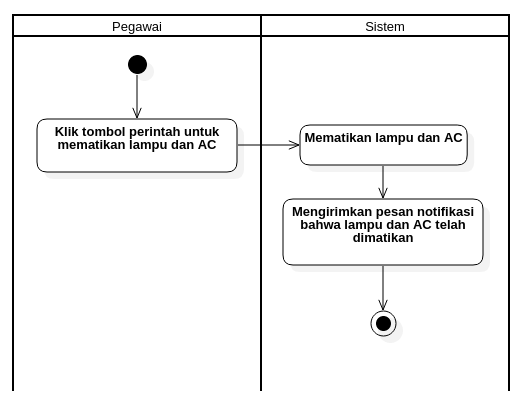
\includegraphics[width=\linewidth]{bab4/img/activity_diagram_mematikan.png}
	}
	\caption{Diagram Aktivitas: Mematikan Lampu dan AC Ruangan}
	\label{figure:activity_2}
\end{figure}

\subsubsection{Desain Sistem Melihat Status Kondisi Lampu dan AC Ruangan}
\tab Seperti fitur-fitur sebelumnya, pengguna yang dapat menggunakan fitur ini hanyalah pengguna yang telah terotorisasi dan terotentikasi. Pengguna dapat menampilkan kondisi lampu dan AC pada sebuah ruangan untuk mengecek apakah ruangan tersebut sedang digunakan atau tidak. Gambar \ref{figure:activity_3} merupakan Diagram aktivitas yang menjelaskan alur untuk menampilkan status kondisi lampu dan AC pada sebuah ruangan.

\begin{figure}[H]
	\centerline {
		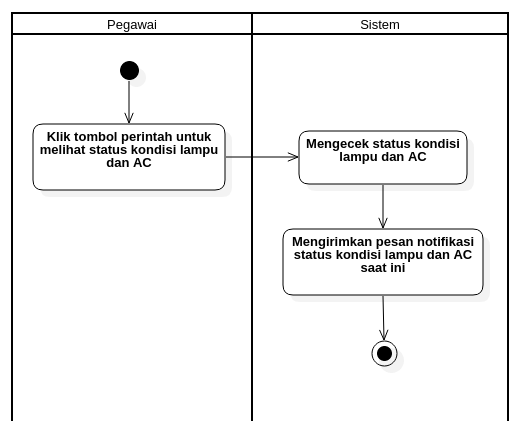
\includegraphics[width=\linewidth]{bab4/img/activity_diagram_melihatstatus.png}
	}
	\caption{Diagram Aktivitas: Melihat Status Kondisi Lampu dan AC Ruangan}
	\label{figure:activity_3}
\end{figure}

\subsubsection{Desain Sistem Melihat Suhu Ruangan}
\tab Pengguna yang dapat menggunakan fitur ini hanyalah pegawai yang telah terotentikasi dan terotorisasi. Pegawai dapat melihat suhu ruangan menggunakan perintah tertentu yang dapat dilihat dalam manual penggunaan bot. Diagram aktivitas pada gambar \ref{figure:activity_4} akan menjelaskan alur untuk menyalakan lampu dan AC ruangan secara lebih jelas.

\begin{figure}[H]
	\centerline {
		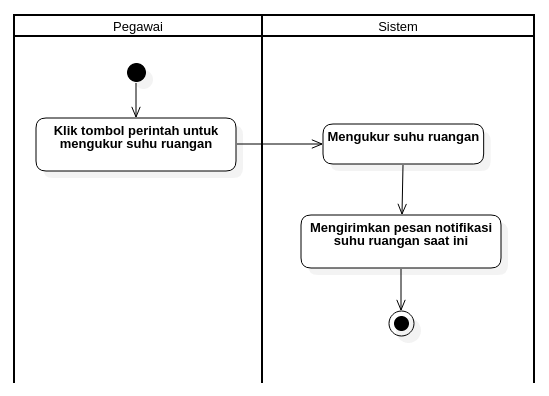
\includegraphics[width=\linewidth]{bab4/img/activity_diagram_mengukursuhu.png}
	}
	\caption{Diagram Aktivitas: Melihat Suhu Ruangan}
	\label{figure:activity_4}
\end{figure}
